\appendix
\chapter{Glossar}

\paragraph{Guest -} a visitor of the website.
\paragraph{User -} the user type relating to the wiki permissions.
\paragraph{Mod -} the user type relating to the wiki permissions. 
\paragraph{Admin -} the user type relating to the wiki permissions. 
\paragraph{(Wiki) Content -} a page in the wiki. Could belong to News, BSI catalogue, articles or archived versions of all of the above.
\paragraph{Article -} a page in the wiki which was created by a user and does not belong to the News or BSI catalogue.
\paragraph{(Wiki) Label -}
\paragraph{(Wiki) Topic -}\todo[inline]{Charlie: open glossar items}
\paragraph{Threat -} as defined by the BSI Grundschutzkatalog (Gef\"ahrdung).
\paragraph{Safeguard -} as defined by the BSI Grundschutzkatalog (Ma\ss nahme).

\chapter{Use case diagrams}

\begin{figure}[h] 
    \centering
    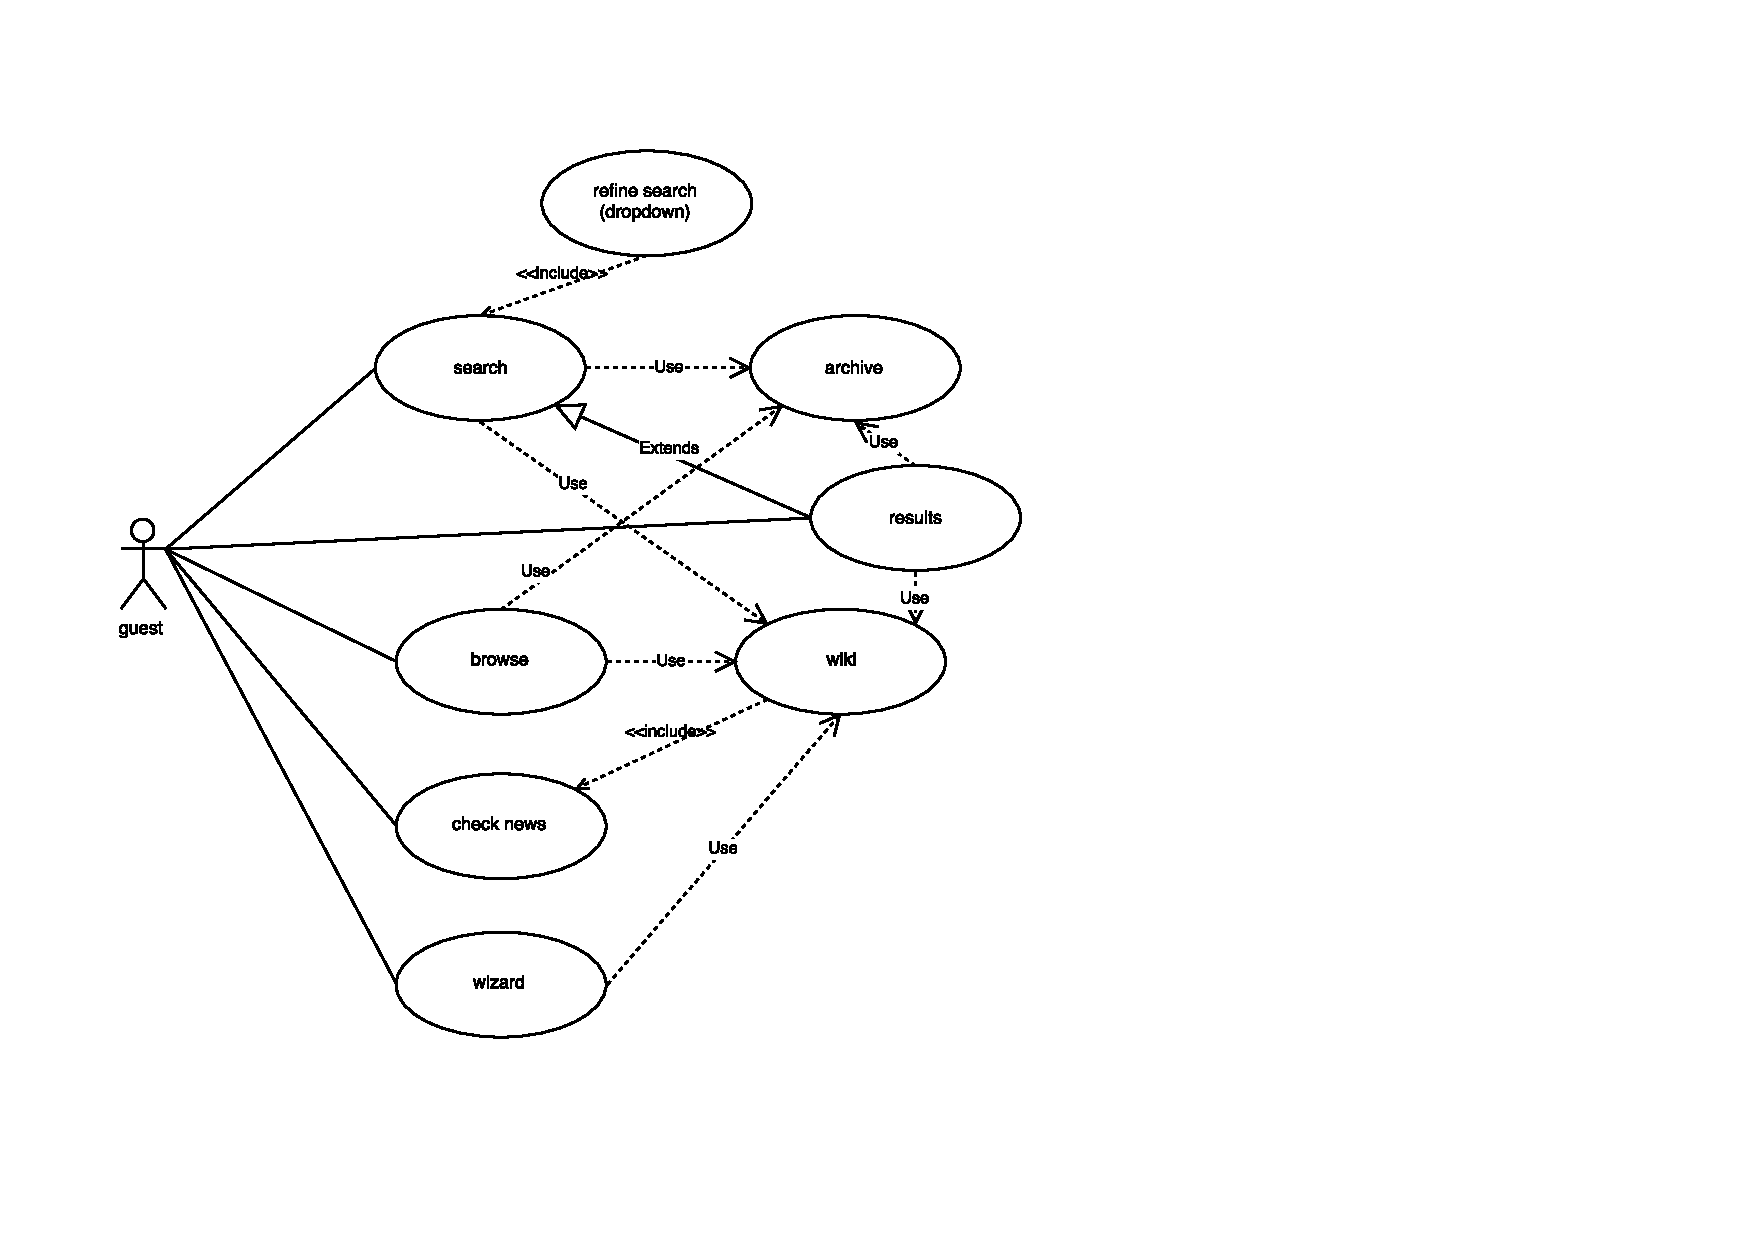
\includegraphics[scale=1.0]{Pictures/Guest}
    \caption{guest - use case}
\end{figure}

\begin{figure}[h] 
    \centering
    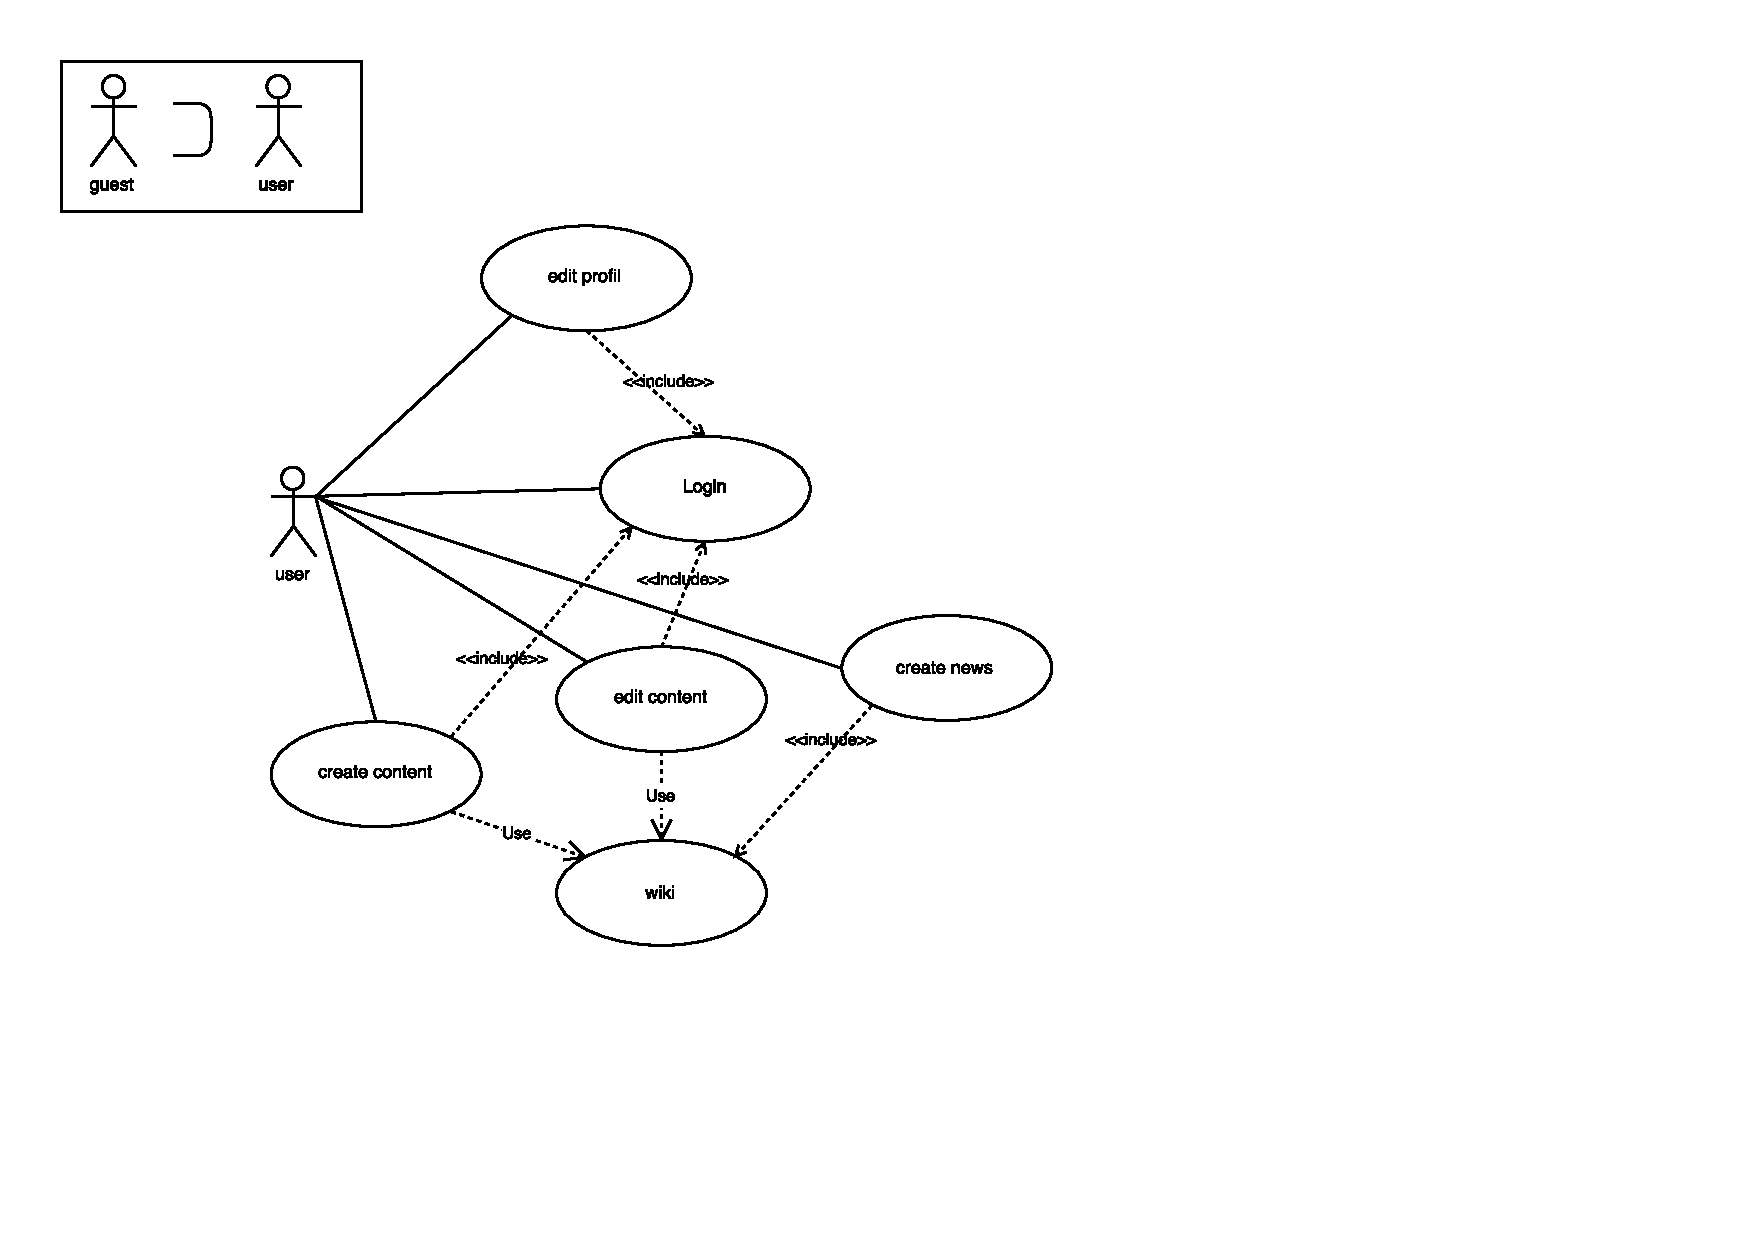
\includegraphics[scale=1.0]{Pictures/User}
    \caption{user - use case}
\end{figure}

\begin{figure}[h] 
    \centering
    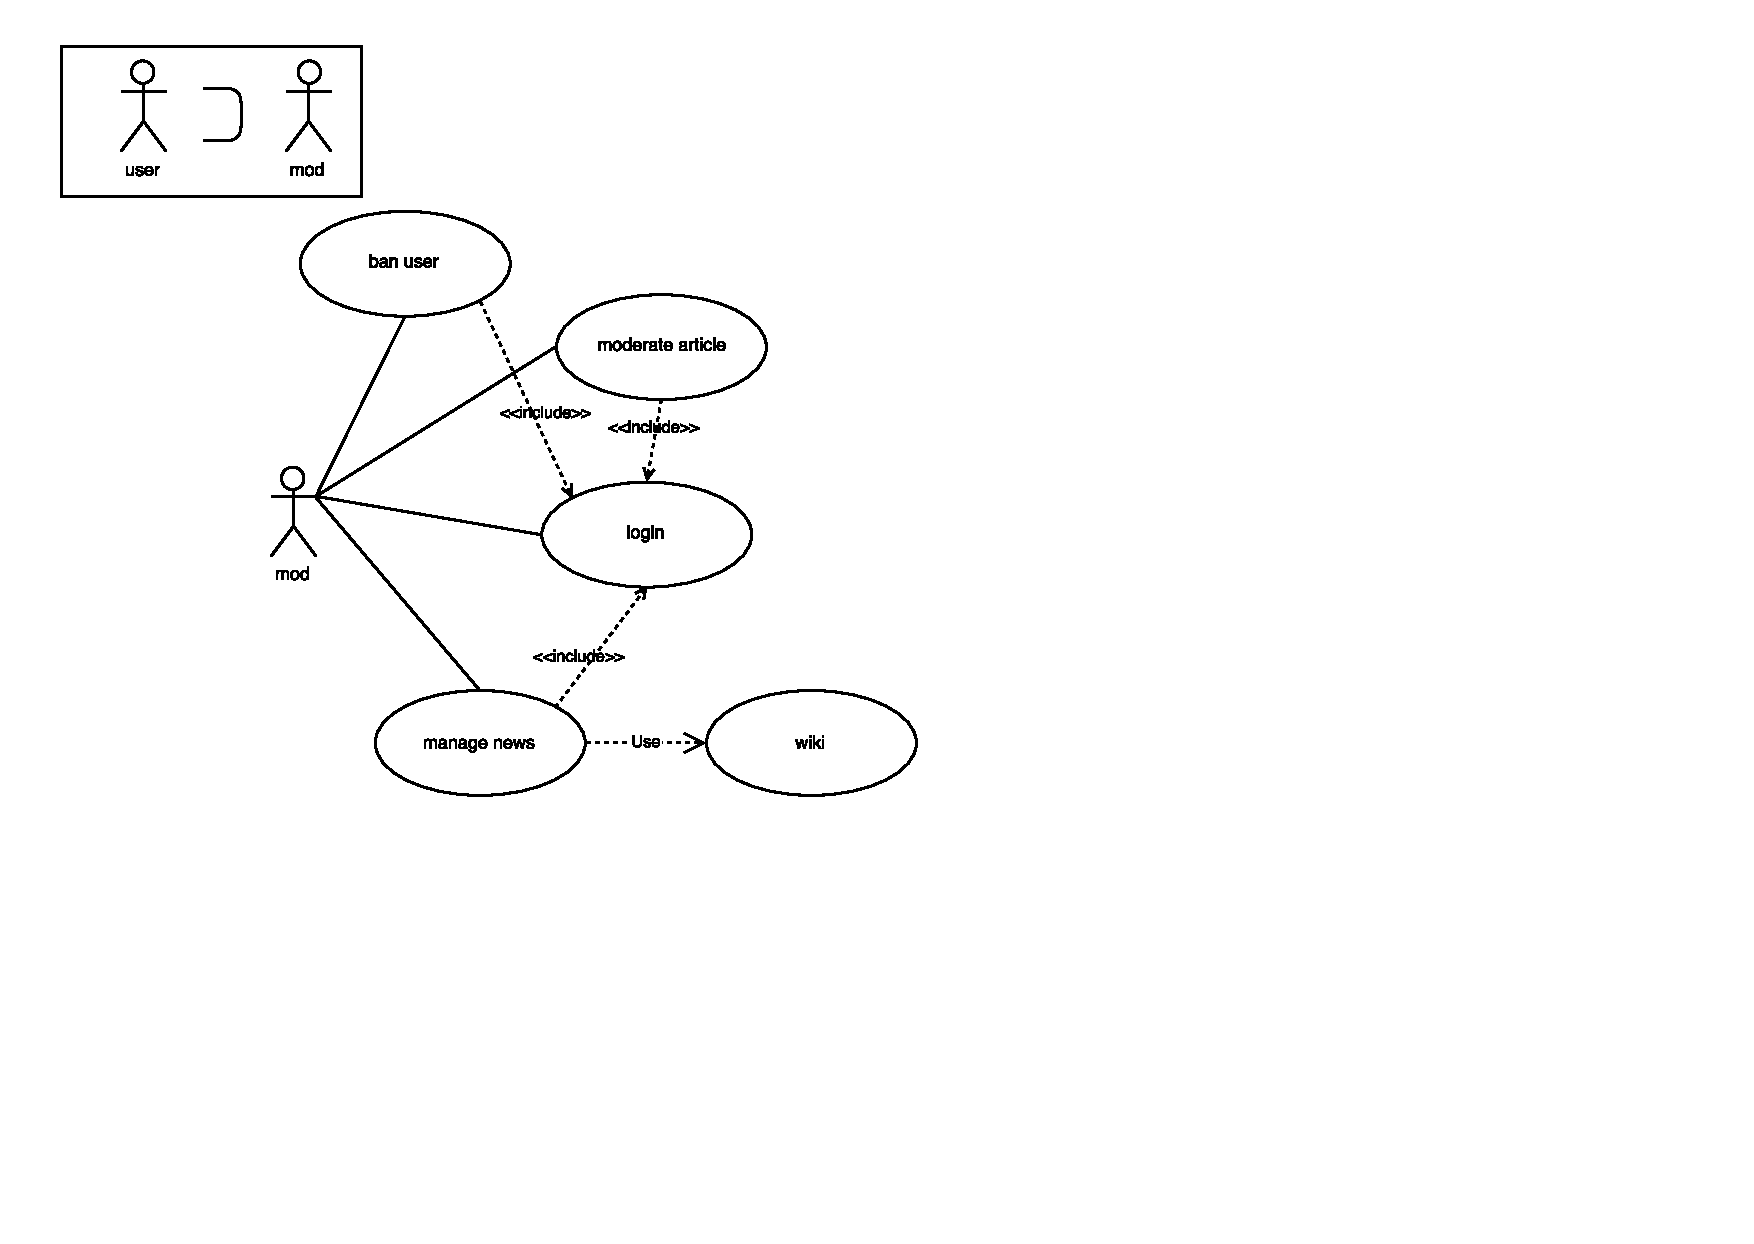
\includegraphics[scale=1.0]{Pictures/Mod}
    \caption{mod - use case}
\end{figure}

\begin{figure}[h] 
    \centering
    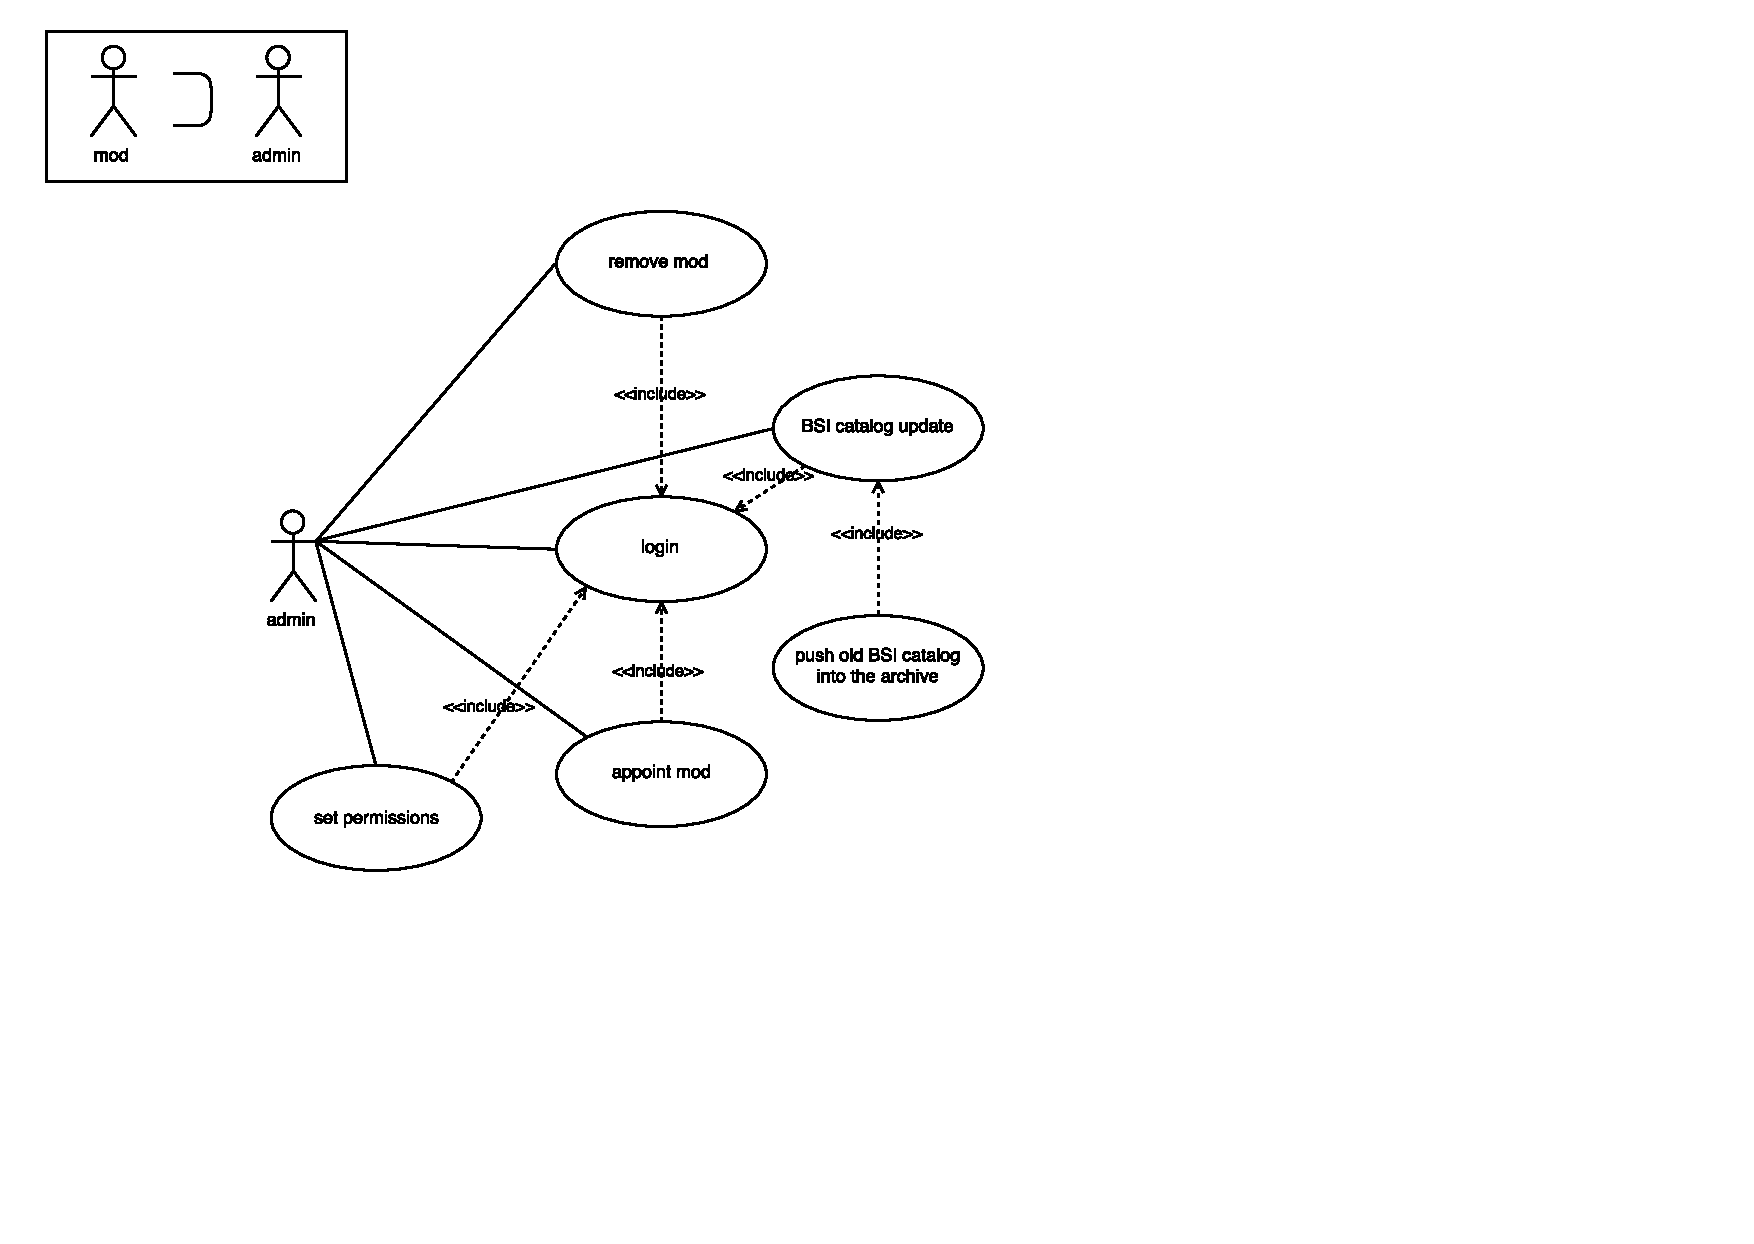
\includegraphics[scale=1.0]{Pictures/Admin}
    \caption{admin - use case}
\end{figure}